\subsubsection{Redux} \label{subsection:4-3-2-1-redux}

\logo{chapter-4/4.3.redux-logo}{Redux logo}

Το Redux\footnote{\url{https://redux.js.org/}} αποτελεί μία βιβλιοθήκη Javascript, η χρήση της οποίας προσφέρει στην εφαρμογή ένα πλήρως διαχειρίσιμο κεντρικό state. 

%TODO: When https://2021.stateofjs.com/en-US/ is available, add to the paragraph above that is the most popular data layer technology (by usage), according to https://2020.stateofjs.com/en-US/technologies/datalayer/ and also add this beautiful chart.

Το Redux συνήθως χρησιμοποιείται για την κατασκευή διεπαφών χρήστη σε συνδύασμό με άλλες βιβλιοθήκες, όπως με την React. Σε αυτήν την περίπτωση, η λειτουργία του UI μπορεί να συνοψιστεί ως εξής:

%TODO: Add proper diagram
\begin{figure}[H]
	\centering
	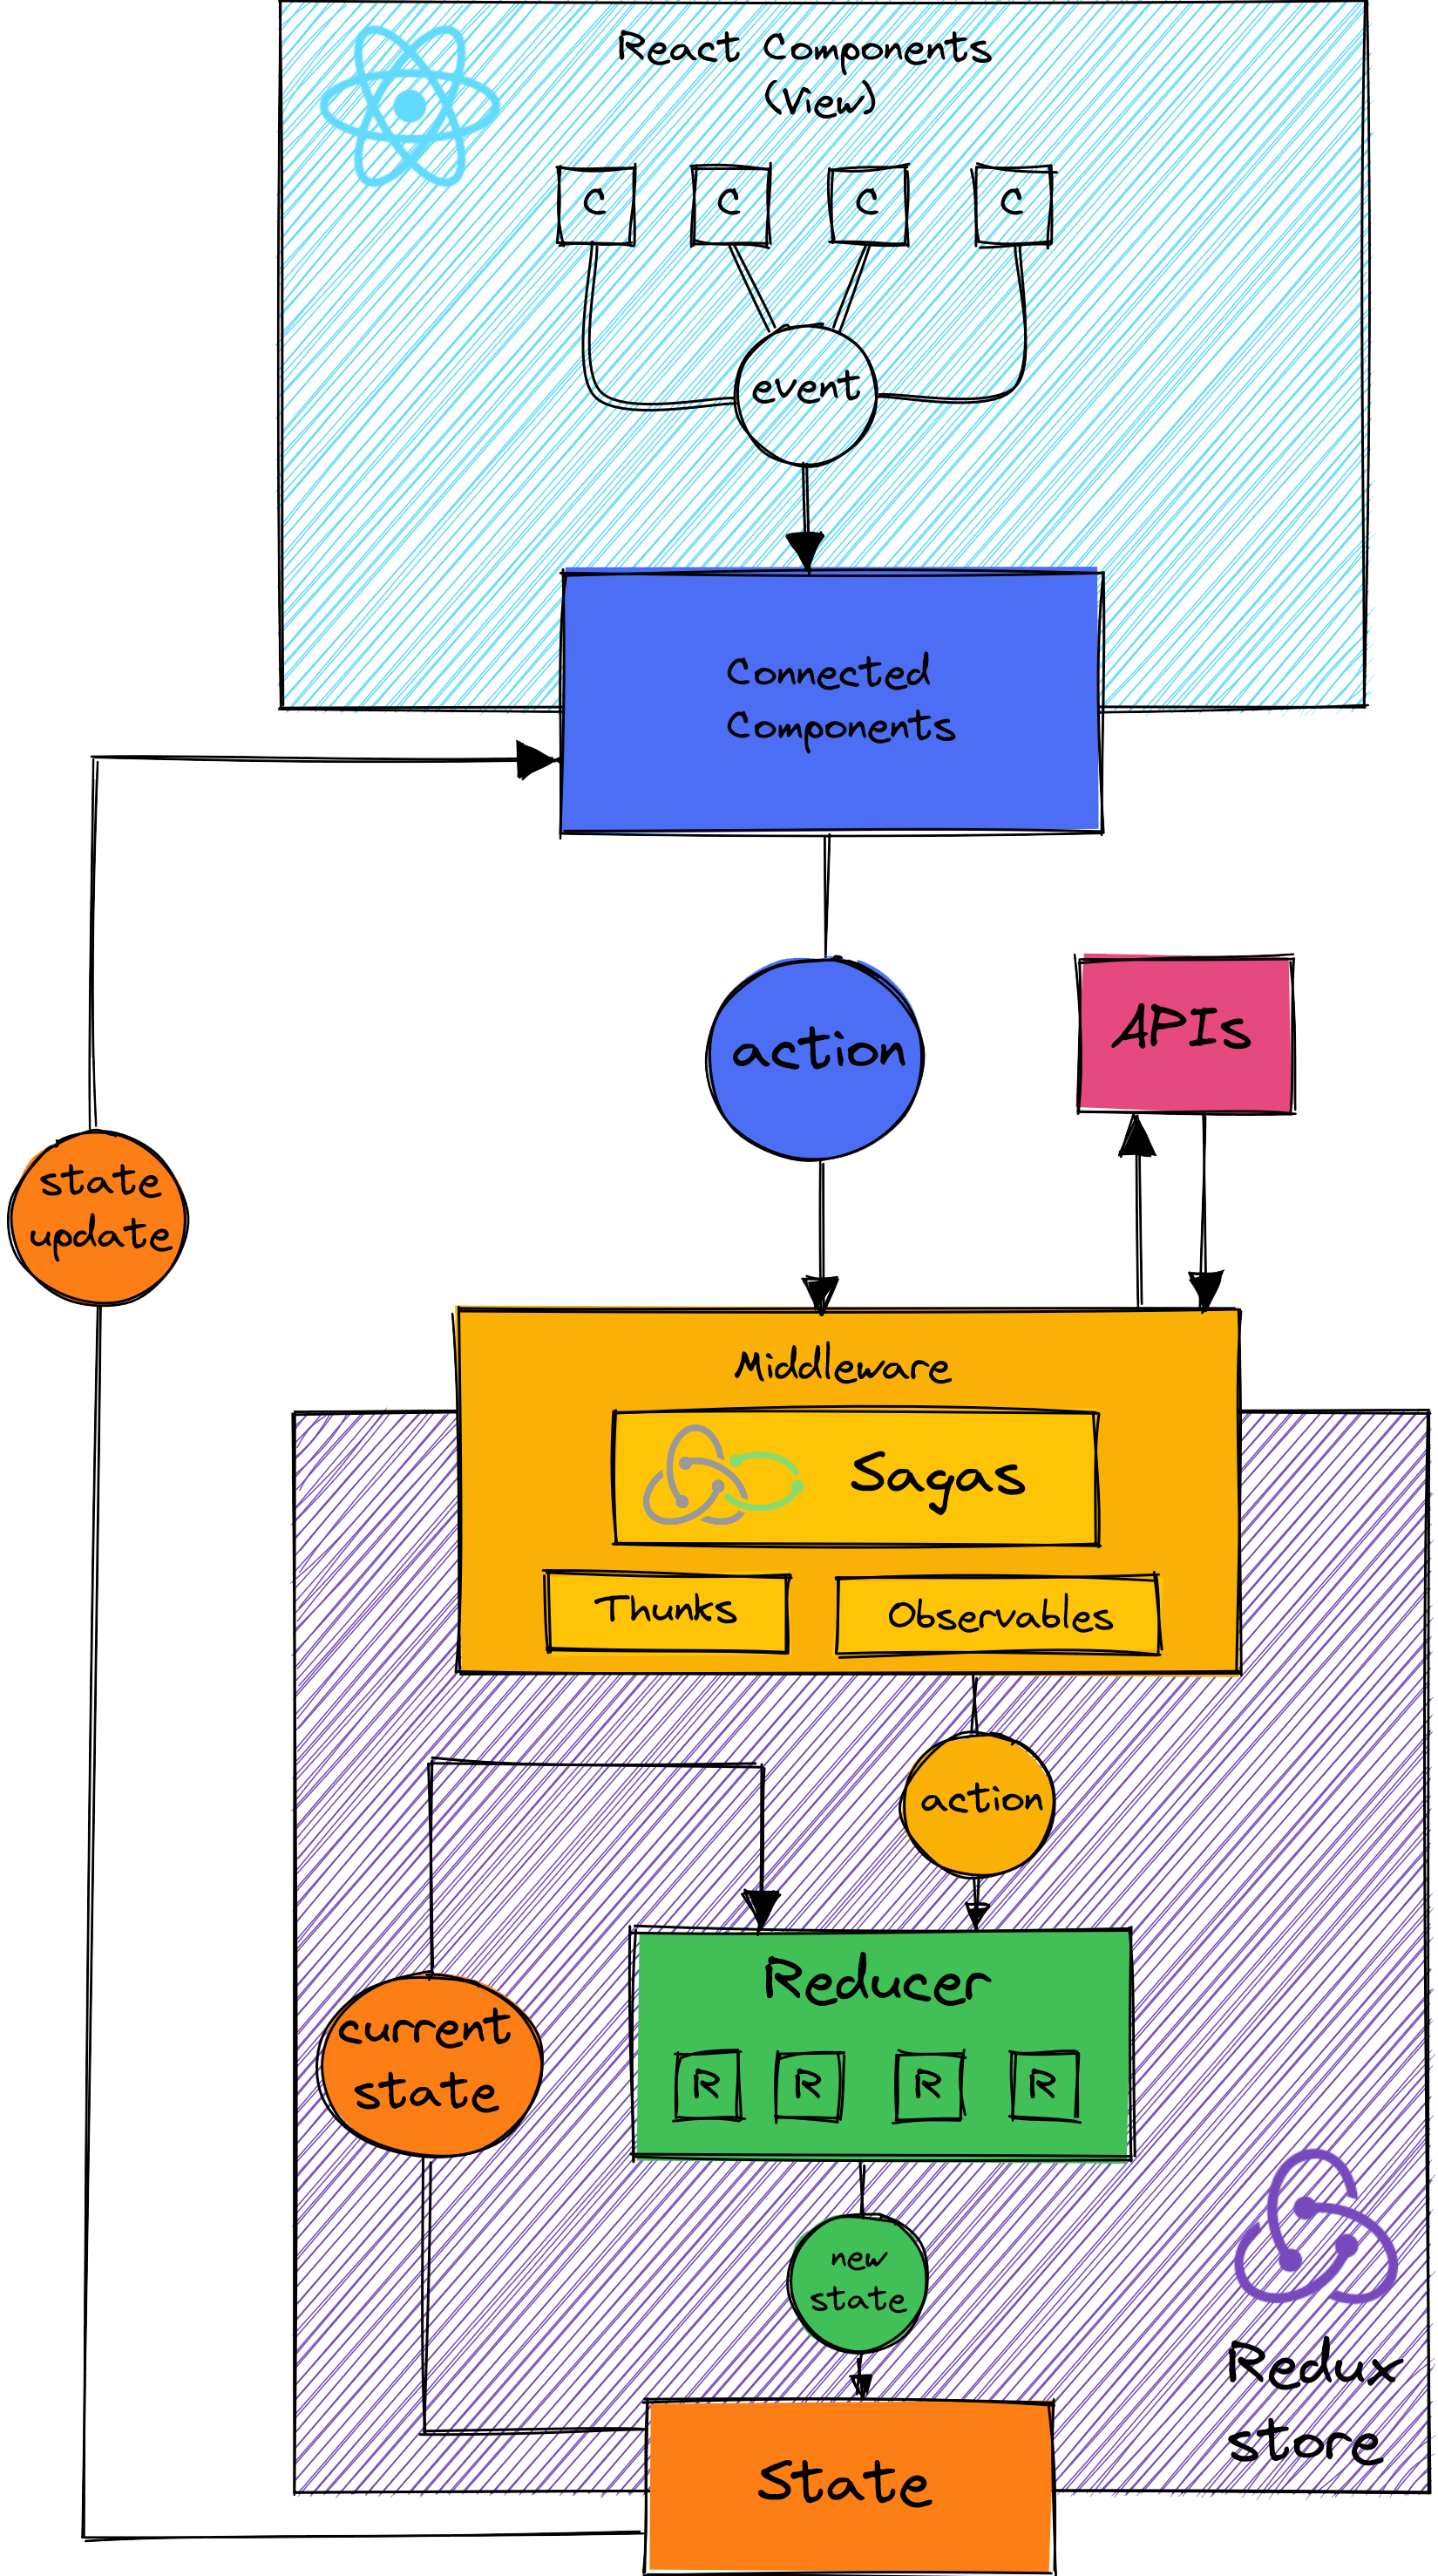
\includegraphics[width=.75\textwidth]{assets/figures/chapter-4/4.3.react-redux}
	\caption{Λειτουργία του Redux σε συνδυασμό με React}
\end{figure}

Το Redux έχει το αποθετήριό του στο GitHub (\url{https://github.com/reduxjs/redux}) και διατίθεται μέσω του μητρώου npm (\url{https://www.npmjs.com/package/redux}).
